\documentclass[conference]{IEEEtran}
\usepackage{graphicx}
\usepackage{float}
\usepackage{subfigure}
\graphicspath{{/home/rafia/Desktop/Paper/}}


\begin{document}

\title{Analyzing NIRCam Test Data}
\author
{\IEEEauthorblockN{Rafia Bushra, Everett Schlawin, Jonathan Fraine}
\IEEEauthorblockA{Department of Astronomy/Steward Observatory\\
University of Arizona}
}
\maketitle



\begin{abstract}
The James Webb Space Telescope (JWST) is a near- and mid-infrared optimized space telescope. It will have unprecedented sensitivity and will be able to see objects fainter and further than those detectable by previous telescopes like the Hubble Space Telescope (HST). Thus, JWST will have tremendous applications in the field of exoplanets. The telescope is equipped with four sensitive instruments: NIRCam, MIRI, NIRSpec and NIRISS. Of these instruments, NIRCam will be the primary imager in the 0.6 - 5 microns wavelength range. At NASA Goddard’s cryogenic vacuum facility in Greenbelt, Maryland, The NIRCam instrument module was used to take extensive images in a controlled environment over several months. The data gathered in the tests is the subject of this article. The images obtained from these tests will be used to create light curves to simulate what happens after JWST launches. This article deals with the extraction process of the time series data and examining different analysis techniques to determine what works best for processing the data.
\end{abstract}



\section{Introduction}
The JWST will revolutionize the field of exoplanetary sciences. The telescope's sensitivity combined with the broad range of wavelength coverage (0.6 - 28 microns) enables it to make accurate measurement of transits. JWST will also look in planetary atmospheres to determine chemical composition and evolution. Most planets however, are quite small compared to their host stars and their atmospheres are even smaller. Thus, understanding atomic and molecular composition in transiting exoplanets requires very precise measurements at precision levels of around 30 parts per million. To achieve that kind of sensitivity, we will need to understand every detail of the telescope, camera and electronics.\\
To understand the details of the telescope and it's camera, the instrument modules have been used to run simulations and gather data. The collected data is converted to fits files, which we will use to extract time series and create light curves. In this paper, we will be describing the steps we took to extract the data, to increase the accuracy of measurements and discuss the methods that worked best in analyzing the data.   



\section{Procedure}
As mentioned above, this paper deals with analyzing NIRCam test data to extract time series and create light curves. Light curve is a plot demonstrating the variation of light received from a source over a certain amount of time. For the test, electrical lamps were used as light source.\\
The first step in creating a light curve is extracting flux and the corresponding time intervals. However, there are some complications in that process e.g. generating separate centers for each image, deciding on an aperture radius, subtracting background noise etc. To properly describe the whole method, we have divided it into small sections and briefly described them below.   


\subsection{Extracting Flux and Time}
This is the first step of creating a light curve.\\
The time for each image in a test is extracted from some information provided in the header of the fits file. Time is calculated using the following formula:
$$Time =  (NGROUP  + 1) * TGROUP * (ON\_NINT - 1)$$
Where, \\
$NGROUP$ = Number groups in an integration\\
$TGROUP$ = Delta time between groups\\
$ON\_NINT$ = INT of total number of NINT in original file\\
These are information that can be found in the header of the respective fits file. \\
Extracting flux involves many small components and thus deserves to be broken down to subdivisions. So the next few subsections will sequentially describe how we extracted the Flux.

\subsubsection{Generating Slope Images}
Flux is calculated in data numbers per second ($DN/s$), so it is a slope calculated from the data. There are different ways to generate slope images.\\
If the files are in .slp format, they can be used as is because the slopes have already been calculated. The .slp files should be used if $NGROUP > 2$ because then there is enough reads for a good fit.\\
If $NGROUP = 2$, the .red formats should be used. The slopes are not calculated and there are 2 reads to calculate the slope from. There are two ways to calculate the slope.\\
The first is called the Slope1 method, also known as CDS (Correlated Double Subtraction). In this method, slope is calculated using the following formula:
$$\frac{(Last Group - First Group)}{(NGROUP-1)*TGROUP}$$
The second method for calculating slope from a .red file is the Slope2 method. Slope is calculated in the following way:
$$\frac{(Last Group - Bias)}{NGROUP*TGROUP}$$
After comparison, we found that the Slope2 method gives better results. This is demonstrated in the figure below.
\begin{figure}[H]
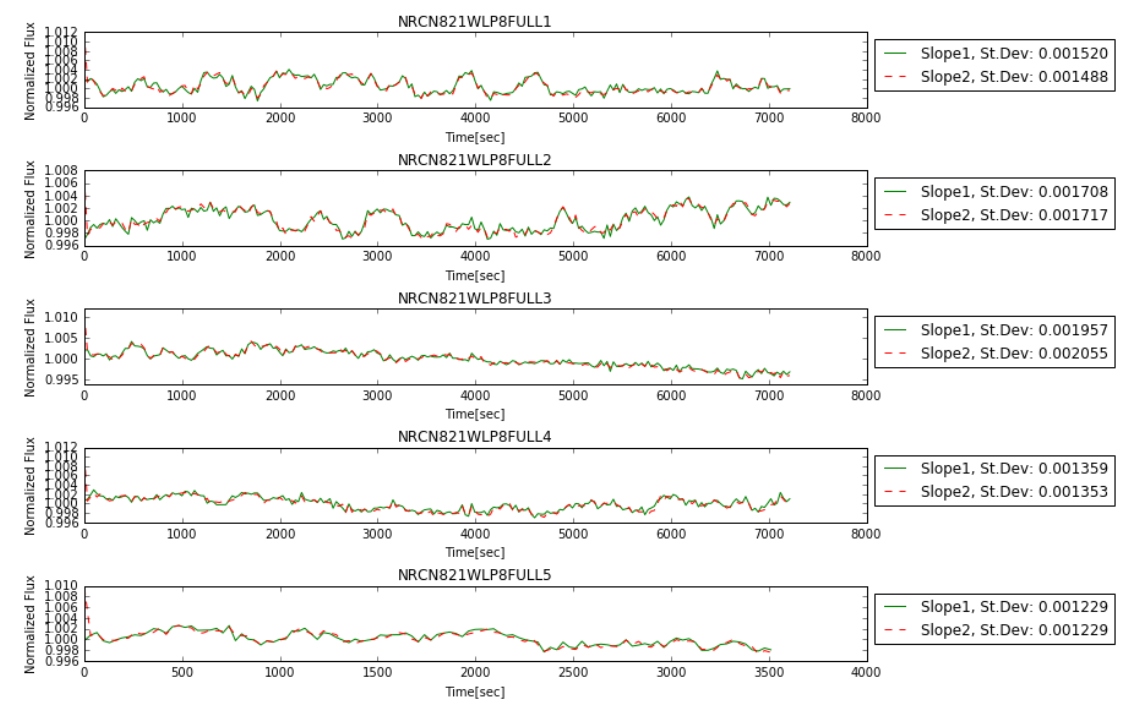
\includegraphics[scale=0.35]{Slopes}
\caption{Plot demonstrating light curves \& standard deviations obtained using Slope1 and Slope2 methods for 5 different tests.}
\label{fig:slopes}
\end{figure}
So wherever applicable, we will be using the Slope2 method.   

\subsubsection{Generating Centers}
For the same test, for a particular detector, expecting all the images to share a common center is a good approximation but not very accurate. So if the model's center is fitted to a Gaussian model, that gives a much closer approximation of an individual image's center. Here is an example Gaussian fit:
\begin{figure}[H]
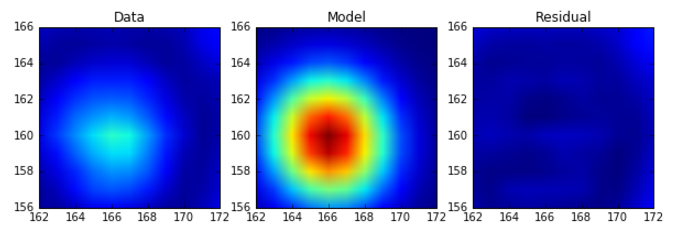
\includegraphics[scale=0.5]{Gaussian}
\caption{Example of Gaussian fitting to an image's center}
\end{figure}
The flux is extracted using circular aperture, for which the center is needed. When extracting flux from each image of a test, their individual center obtained from Gaussian fitting will be used.  

\subsubsection{Radius Testing}
The circular aperture function used for flux extraction also requires a radius. This radius is the source radius. The radius has to be chosen so that the measured error or standard deviation is minimum. For this, we extract the flux multiple times using varying radius values and calculate standard deviations. Here is plot showing how the best radius is chosen:
\begin{figure}[H]
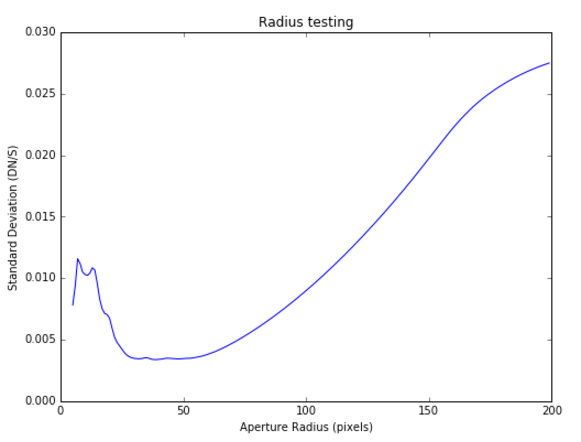
\includegraphics[scale=0.5]{Radius}
\caption{A plot of Standard Deviation Vs. Aperture Radius. The minimum of the curve gives the best aperture radius}
\end{figure}


\subsubsection{Subtracting Background}
Other than the light received from the source, there is usually some background noise that we have to account for in order to get more accurate results. For this we are using an annulus out side the source to subtract. The annulus has an inner radius and an outer radius. So now, there are three different radii to consider: source radius, inner radius (BG subtraction) and inner radius (BG subtraction). The best combination of these three is determined through a radius test. 
\begin{figure}[H]
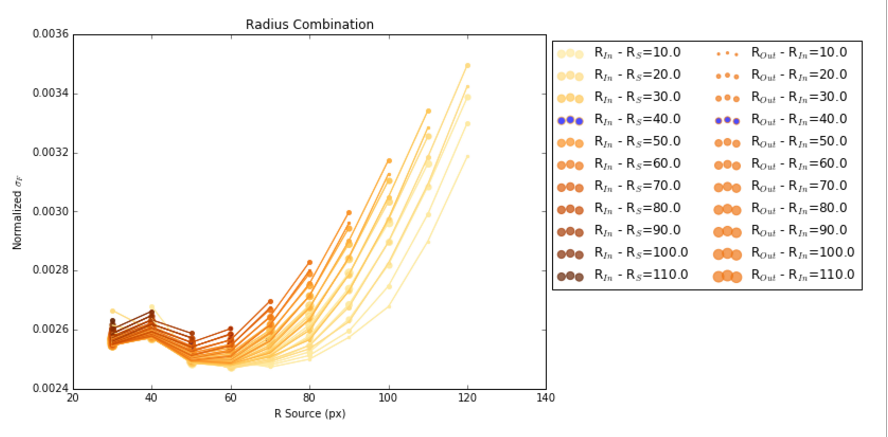
\includegraphics[scale=0.45]{Combo}
\caption{A plot of Standard Deviation Vs. Source Radius for different combinations of inner and out radii. The minimum of the curve gives the best combination}
\end{figure}


\begin{figure}[H]
    \centering
    \begin{subfigure}{1}
        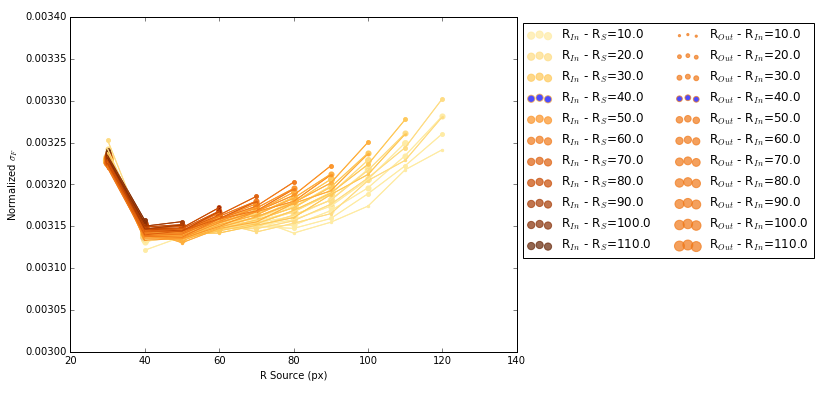
\includegraphics[scale = 0.5]{Radius_640}
        \caption{SUB640}
    \end{subfigure}

    \begin{subfigure}{2}
        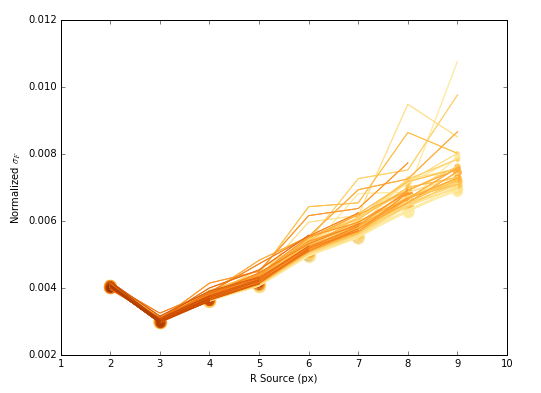
\includegraphics[scale=0.6]{Radius_CLR}
        \caption{CLRSUB}
    \end{subfigure}
\end{figure}
 
 
\subsection{Fitting Data To A 1D-Linear Model}
In order to get the proper standard deviation, the data is fit to a linear model to remove any trend. The data is then divided by the line to get a "de-trended" time series. Here is an example of a linear best fit:
\begin{figure}[H]
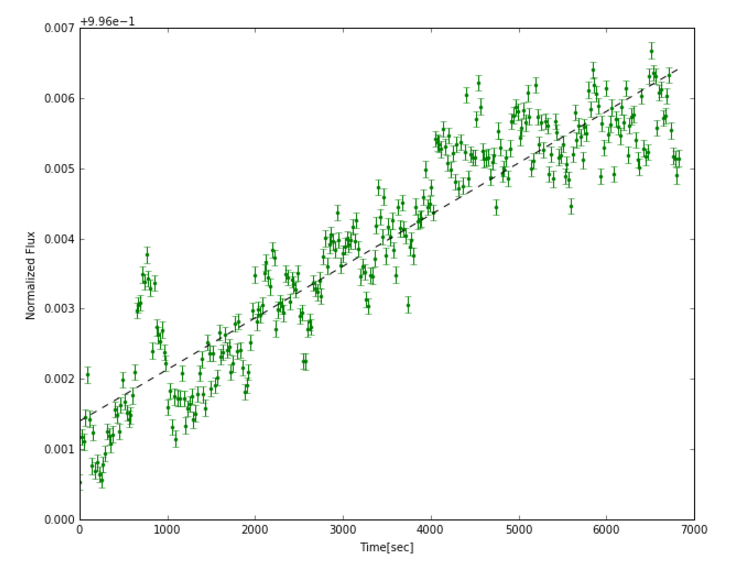
\includegraphics[scale=0.4]{Line}
\caption{An example linear best fit.}
\end{figure} 


\subsection{Calculating Ideal Noise and Measured Noise}
The final step in analyzing any test data is calculating the ideal noise and measured noise. Ideal noise is calculated by $$\sigma_F = \frac{\sqrt{Flux*Time*Gain}}{Time*Gain}$$
The measured noise is the standard deviation of the data. The measured noise (standard deviation) is plotted with time to get a better view of the data. here is an example plot:
\begin{figure}[H]
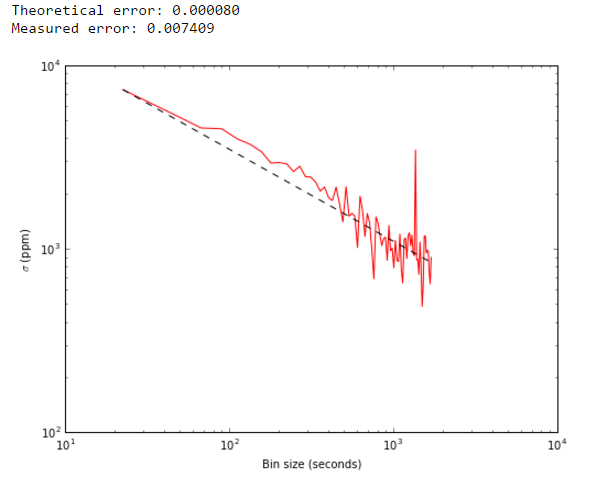
\includegraphics[scale=0.55]{RMS}
\caption{RMS Vs. Time plot to visualize measured noise}
\end{figure}



\section{Correction Methods}
There are 3 different correction methods applied to each test: Inter pixel capacitance(IPC) correction, Linearity correction and Flat Fielding. Their combination is denoted with 3 letters (either M(minus, not applied) or P(plus), applied). We tested a few tests to see which combination gives minimum standard deviation and found that the MMM (i.e. no correction method was applied) tests gave the best results. Here is the result we found:  
\begin{figure}[H]
    \centering
    \begin{subfigure}{1}
        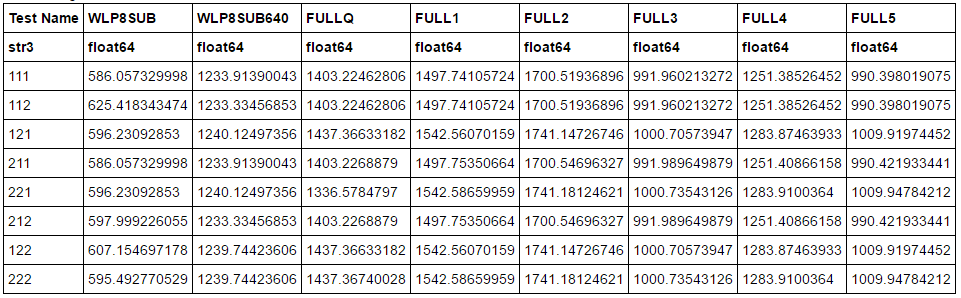
\includegraphics[width=8cm,height=10cm,keepaspectratio]{correction}
        \caption{Table showing the standard deviations for different tests. In the test name column, '1' stands for 'M' and '2' stands for 'P'. E.g. '121' is equivalent to 'MPM'}
    \end{subfigure}

    \begin{subfigure}{2}
        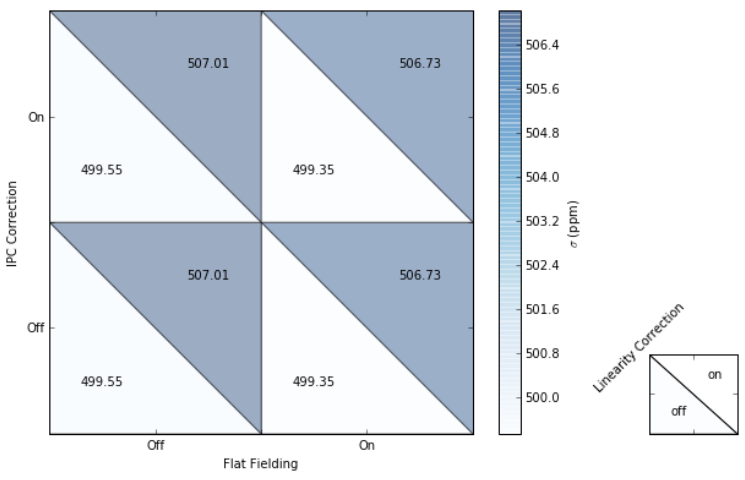
\includegraphics[scale=0.6]{correction1}
        \caption{A plot showing how standard deviation vary with correction method combinations}
    \end{subfigure}
\end{figure}


\begin{figure}[H]
    \centering
    \begin{subfigure}{1}
        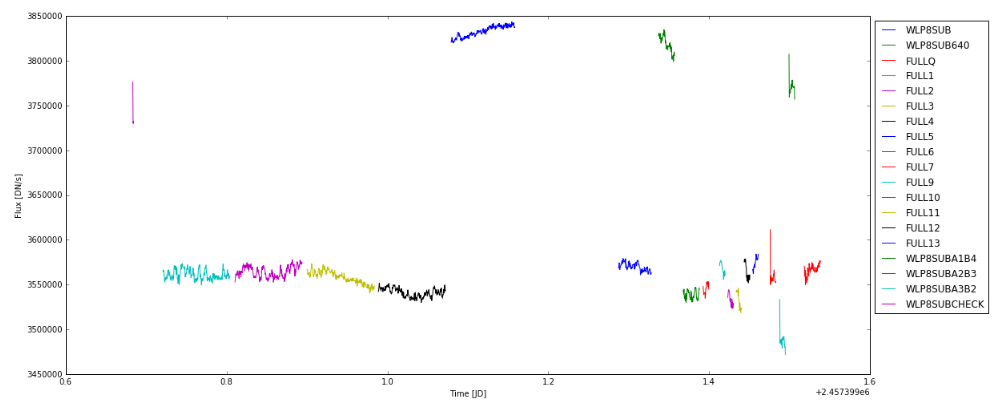
\includegraphics[scale = 0.3]{MMM}
        \caption{MMM}
    \end{subfigure}

    \begin{subfigure}{2}
        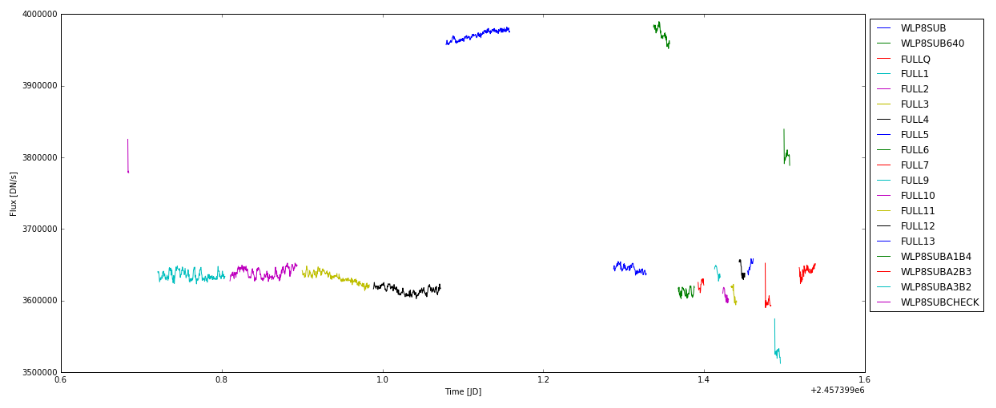
\includegraphics[scale=0.3]{PPP}
        \caption{PPP}
    \end{subfigure}
\end{figure}


\section{Different NIRCam Tests}
In the previous section, we discussed the general method of analyzing a test and gave example plots and curves. In this section we will provide the data analysis of actual tests as obtained by the methods described earlier. For each test, the extracted time series (for a and b detectors separately \& averaged), the averaged light curve with housing temperatures, linear best fit with ideal noise and measured noise vs. time plot will be provided. We average the light curves from two detectors because they are anti-correlated. 


\subsection{Test 1: WLP8SUB} 
\begin{figure}[H]
    \centering
    \begin{subfigure}{1}
        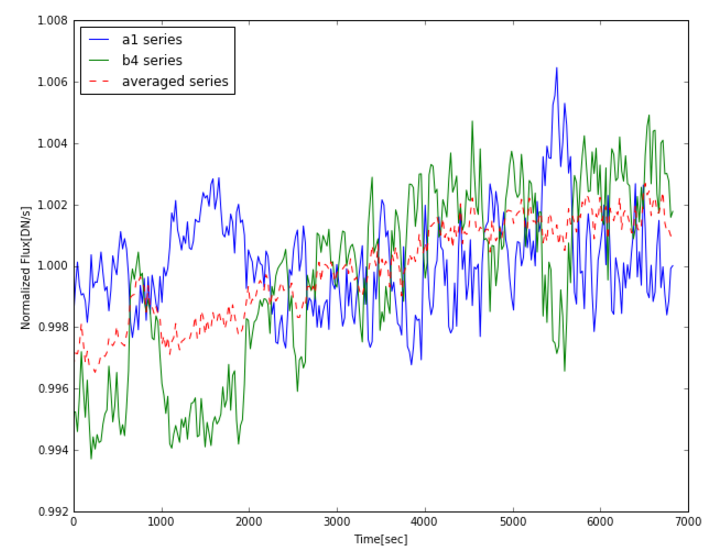
\includegraphics[scale=0.4]{ts_test1}
        \caption{Light curves of a1 series, b4 series and their average}
    \end{subfigure}

    \begin{subfigure}{2}
        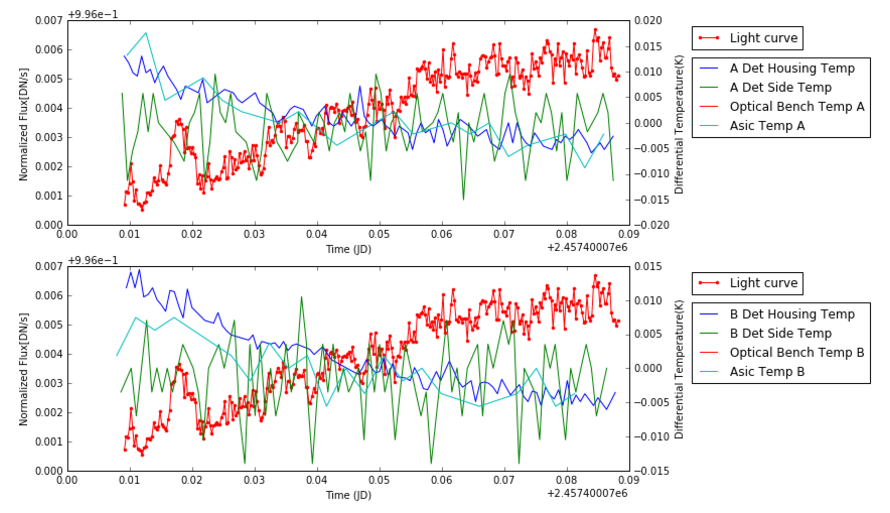
\includegraphics[scale=0.4]{temp_test1}
        \caption{The averaged light curve compared with detector temperatures}
    \end{subfigure}
   
    \begin{subfigure}{3}
        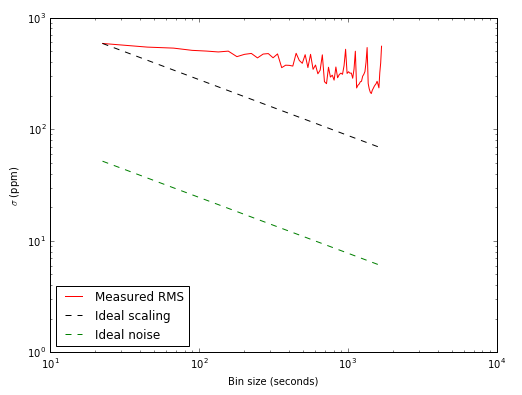
\includegraphics[scale=0.6]{rms_test1}
        \caption{RMS Vs. Bin size}
    \end{subfigure}
    \caption{Analysis of Test 1: WLP8SUB}
\end{figure}


\subsection{Test 2: WLP8SUB640} 
\begin{figure}[H]
    \centering
    \begin{subfigure}{1}
        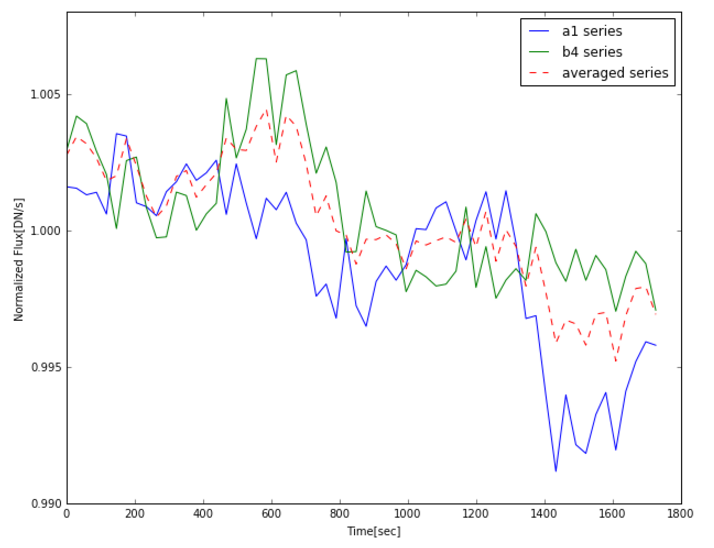
\includegraphics[scale=0.4]{ts_test2}
        \caption{Light curves of a1 series, b4 series and their average}
    \end{subfigure}

    \begin{subfigure}{2}
        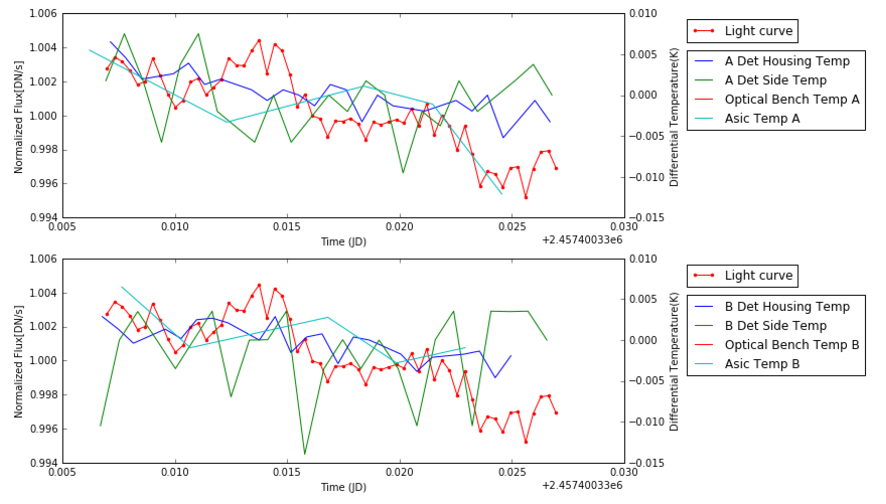
\includegraphics[scale=0.4]{temp_test2}
        \caption{The averaged light curve compared with detector temperatures}
    \end{subfigure}
   
    \begin{subfigure}{3}
        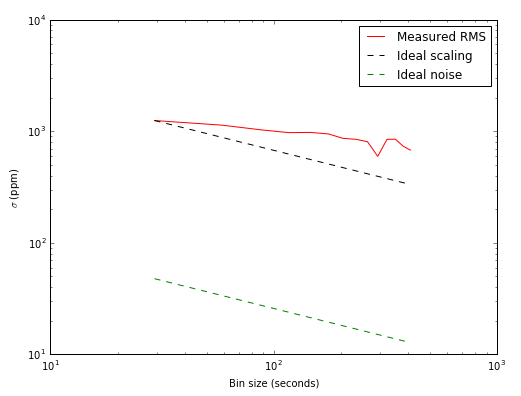
\includegraphics[scale=0.6]{rms_test2}
        \caption{RMS Vs. Bin size}
    \end{subfigure}
    \caption{Analysis of Test 2: WLP8SUB640}
\end{figure}


\subsection{Test 3: FULL0} 
\begin{figure}[H]
    \centering
    \begin{subfigure}{1}
        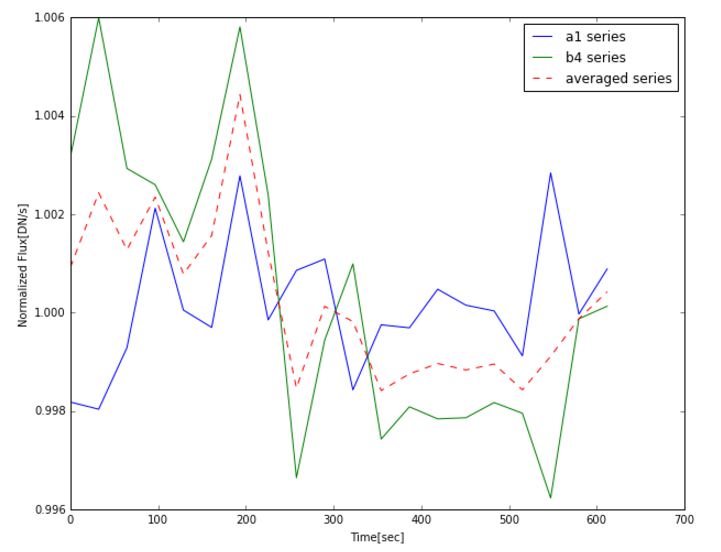
\includegraphics[scale=0.4]{ts_test3}
        \caption{Light curves of a1 series, b4 series and their average}
    \end{subfigure}

    \begin{subfigure}{2}
        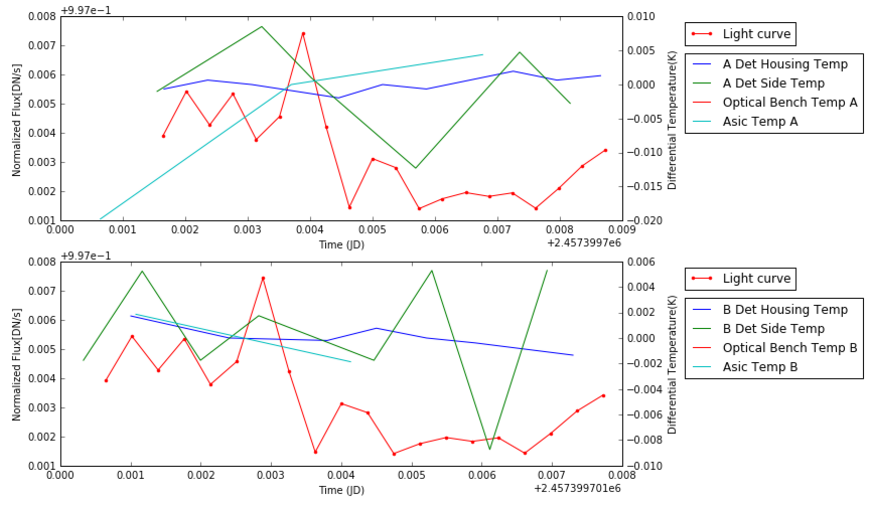
\includegraphics[scale=0.4]{temp_test3}
        \caption{The averaged light curve compared with detector temperatures}
    \end{subfigure}
   
    \begin{subfigure}{3}
        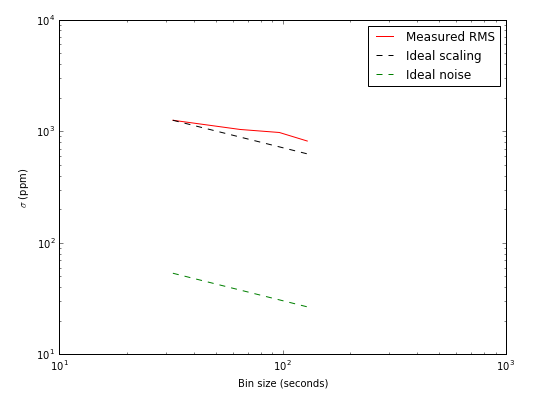
\includegraphics[scale=0.6]{rms_test3}
        \caption{RMS Vs. Bin size}
    \end{subfigure}
    \caption{Analysis of Test 3: FULL0}
\end{figure}


\subsection{Test 4: FULL1} 
\begin{figure}[H]
    \centering
    \begin{subfigure}{1}
        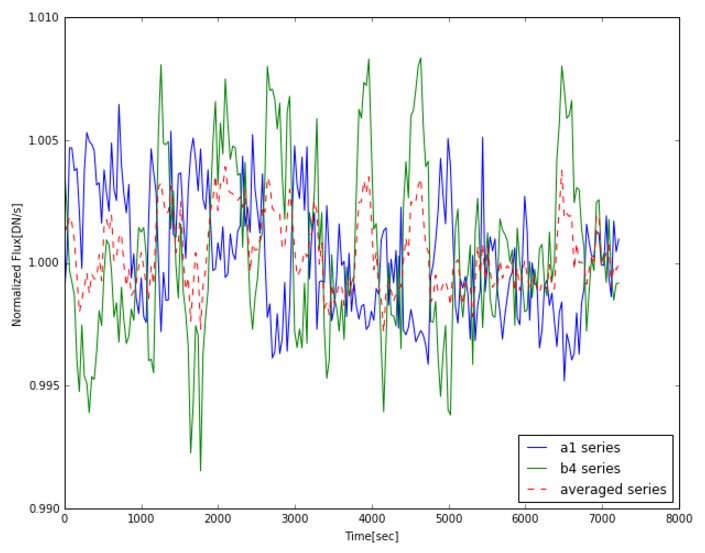
\includegraphics[scale=0.4]{ts_test4}
        \caption{Light curves of a1 series, b4 series and their average}
    \end{subfigure}

    \begin{subfigure}{2}
        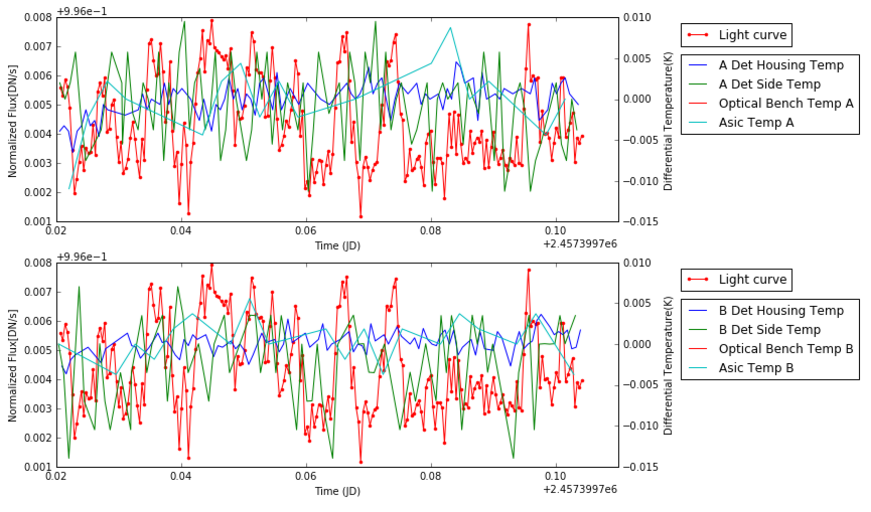
\includegraphics[scale=0.4]{temp_test4}
        \caption{The averaged light curve compared with detector temperatures}
    \end{subfigure}
   
    \begin{subfigure}{3}
        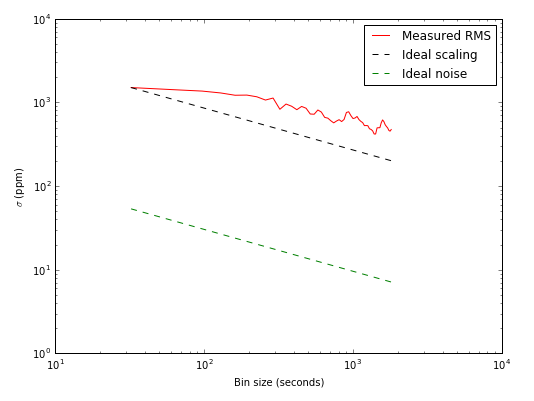
\includegraphics[scale=0.6]{rms_test4}
        \caption{RMS Vs. Bin size}
    \end{subfigure}
    \caption{Analysis of Test 4: FULL1}
\end{figure}


\subsection{Test 5: FULL2} 
\begin{figure}[H]
    \centering
    \begin{subfigure}{1}
        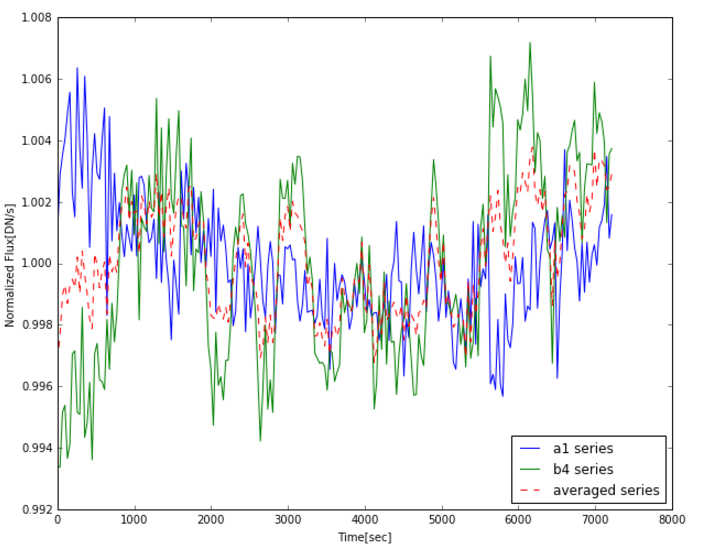
\includegraphics[scale=0.4]{ts_test5}
        \caption{Light curves of a1 series, b4 series and their average}
    \end{subfigure}

    \begin{subfigure}{2}
        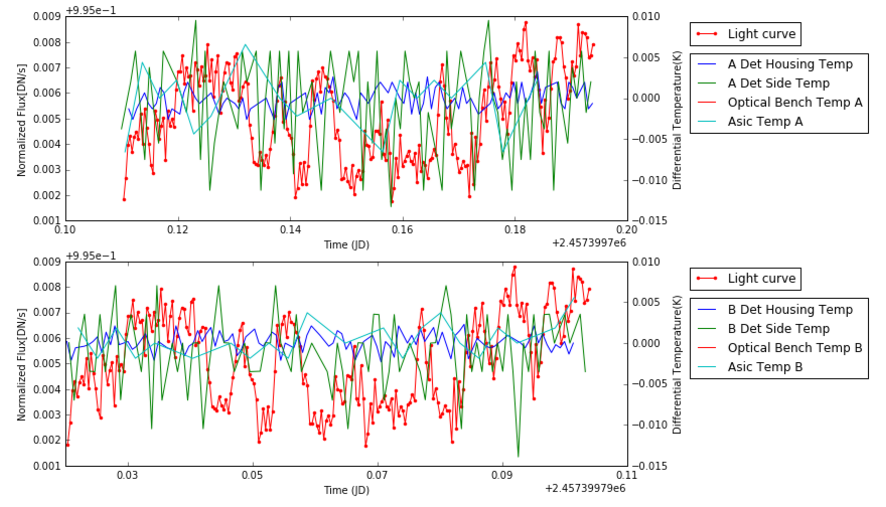
\includegraphics[scale=0.4]{temp_test5}
        \caption{The averaged light curve compared with detector temperatures}
    \end{subfigure}
   
    \begin{subfigure}{3}
        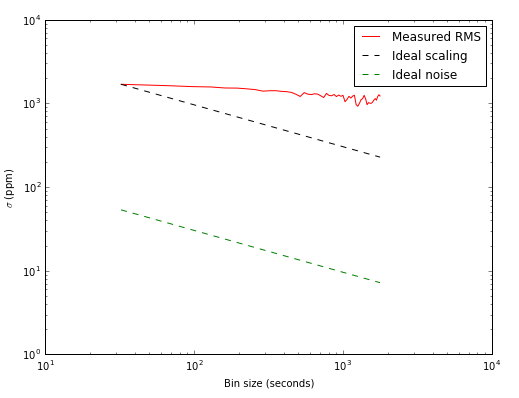
\includegraphics[scale=0.6]{rms_test5}
        \caption{RMS Vs. Bin size}
    \end{subfigure}
    \caption{Analysis of Test 5: FULL2}
\end{figure}


\subsection{Test 6: FULL3} 
\begin{figure}[H]
    \centering
    \begin{subfigure}{1}
        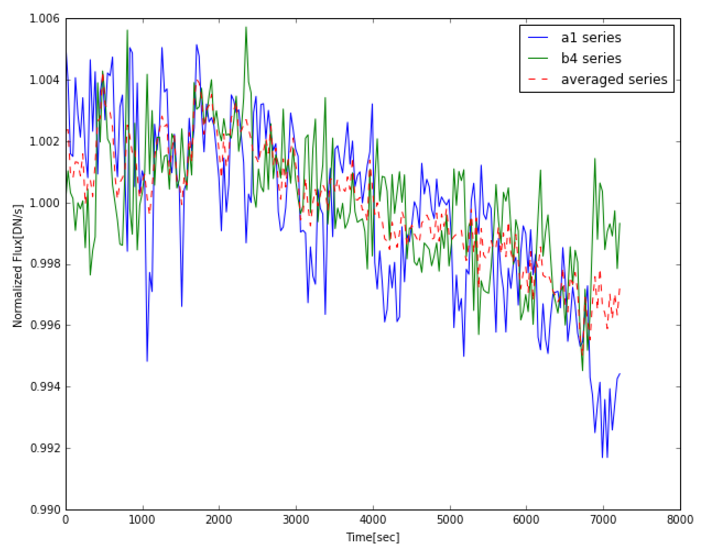
\includegraphics[scale=0.4]{ts_test6}
        \caption{Light curves of a1 series, b4 series and their average}
    \end{subfigure}

    \begin{subfigure}{2}
        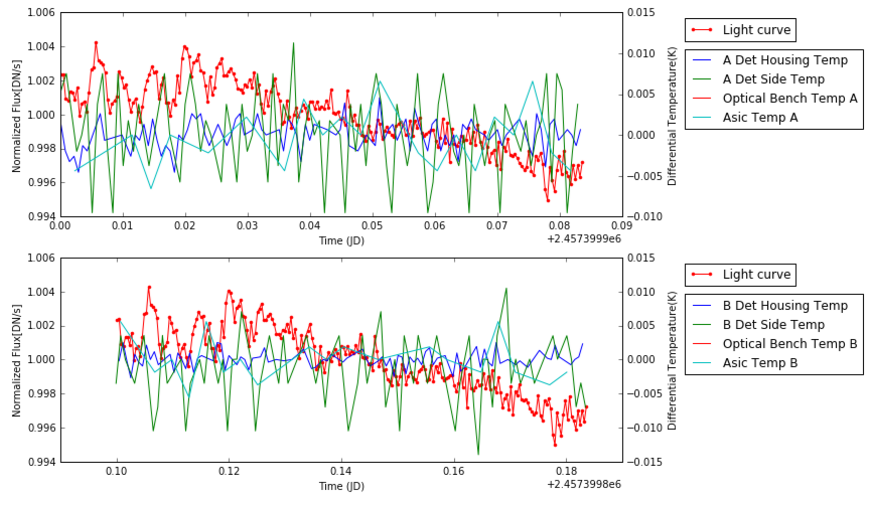
\includegraphics[scale=0.4]{temp_test6}
        \caption{The averaged light curve compared with detector temperatures}
    \end{subfigure}
   
    \begin{subfigure}{3}
        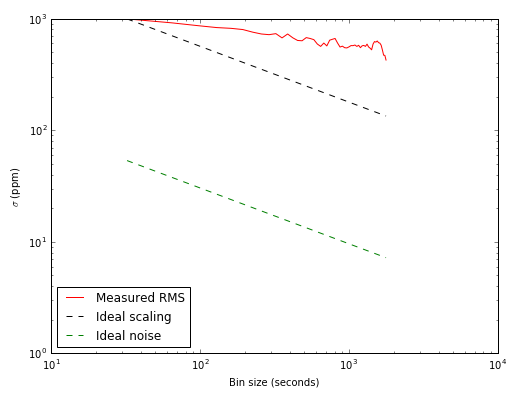
\includegraphics[scale=0.6]{rms_test6}
        \caption{RMS Vs. Bin size}
    \end{subfigure}
    \caption{Analysis of Test 6: FULL3}
\end{figure}


\subsection{Test 7: FULL4} 
\begin{figure}[H]
    \centering
    \begin{subfigure}{1}
        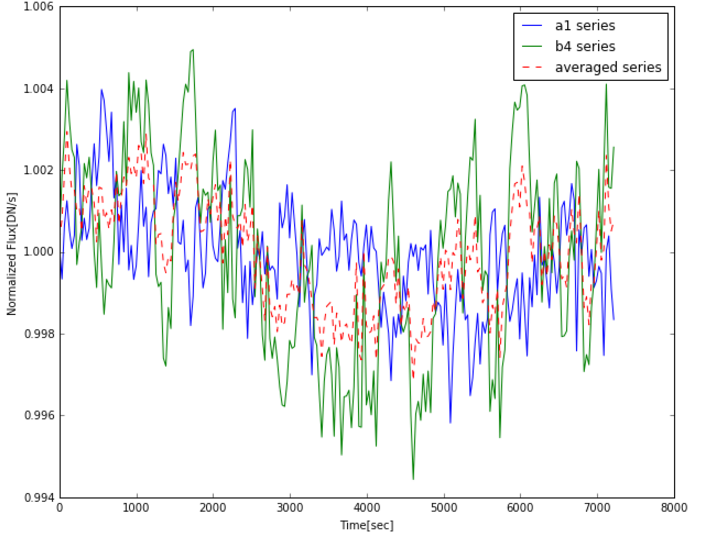
\includegraphics[scale=0.4]{ts_test7}
        \caption{Light curves of a1 series, b4 series and their average}
    \end{subfigure}

    \begin{subfigure}{2}
        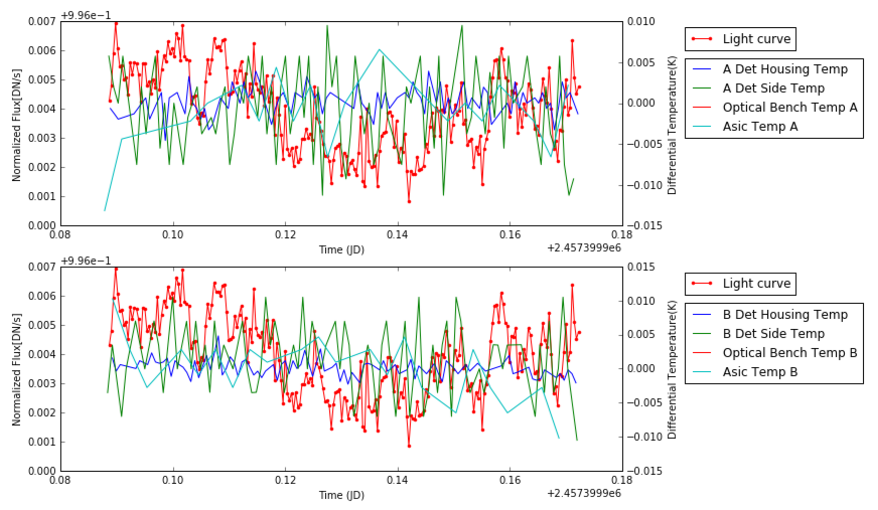
\includegraphics[scale=0.4]{temp_test7}
        \caption{The averaged light curve compared with detector temperatures}
    \end{subfigure}
   
    \begin{subfigure}{3}
        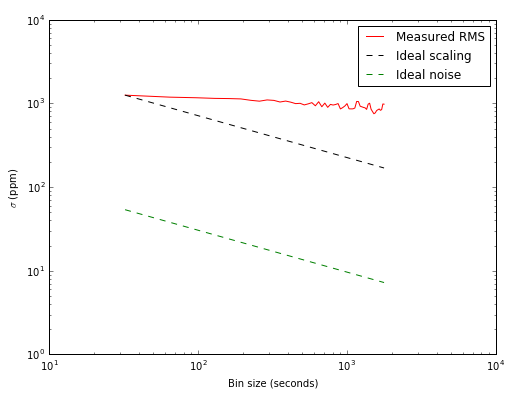
\includegraphics[scale=0.6]{rms_test7}
        \caption{RMS Vs. Bin size}
    \end{subfigure}
    \caption{Analysis of Test 7: FULL4}
\end{figure}


\subsection{Test 8: FULL5} 
\begin{figure}[H]
    \centering
    \begin{subfigure}{1}
        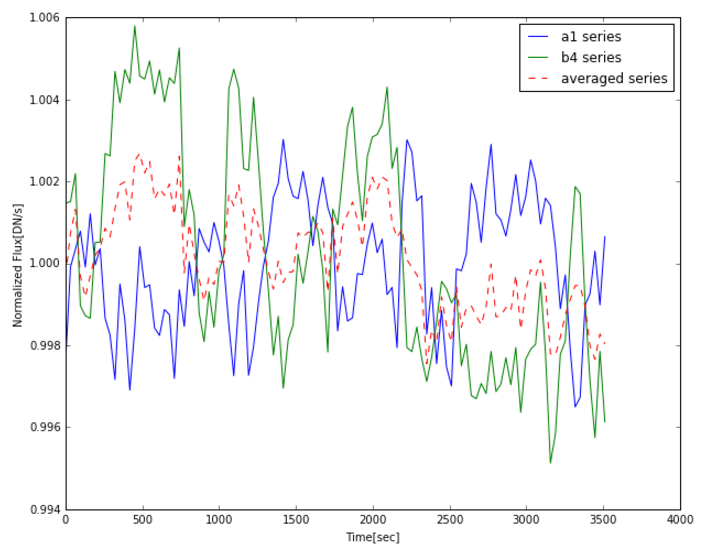
\includegraphics[scale=0.4]{ts_test8}
        \caption{Light curves of a1 series, b4 series and their average}
    \end{subfigure}

    \begin{subfigure}{2}
        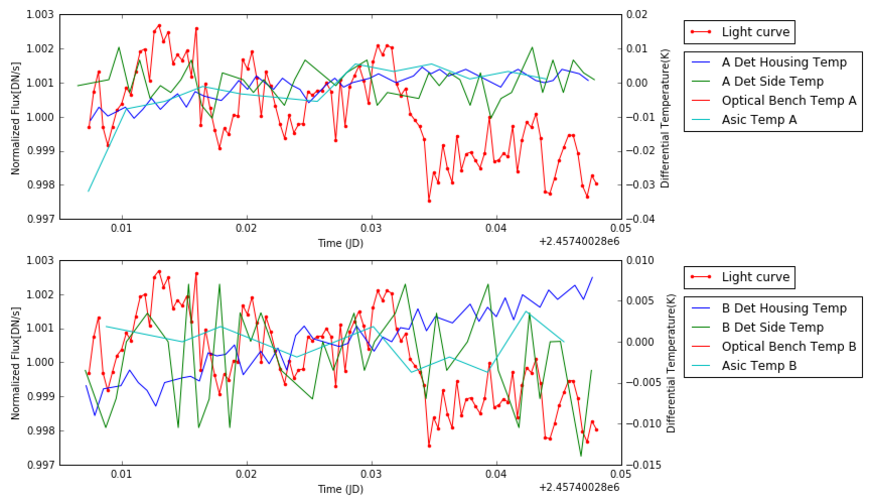
\includegraphics[scale=0.4]{temp_test8}
        \caption{The averaged light curve compared with detector temperatures}
    \end{subfigure}
   
    \begin{subfigure}{3}
        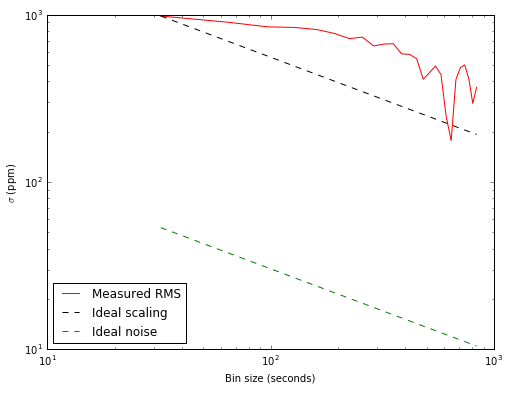
\includegraphics[scale=0.6]{rms_test8}
        \caption{RMS Vs. Bin size}
    \end{subfigure}
    \caption{Analysis of Test 8: FULL5}
\end{figure}


\subsection{Test 9: FULL6} 
\begin{figure}[H]
    \centering
    \begin{subfigure}{1}
        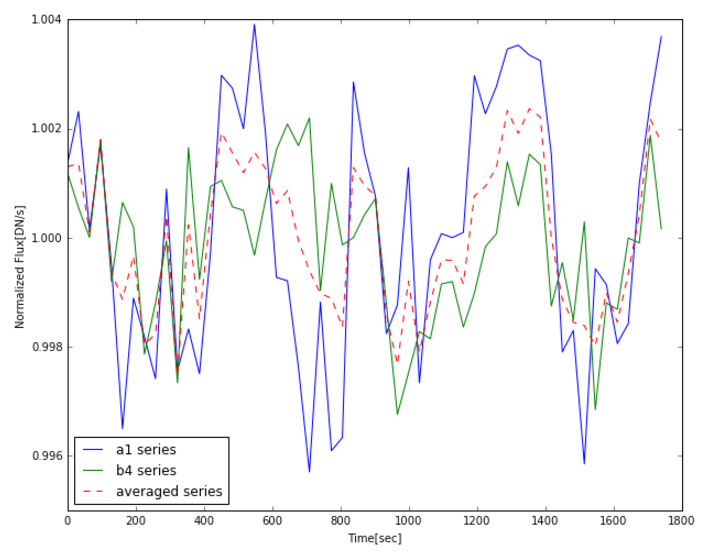
\includegraphics[scale=0.4]{ts_test9}
        \caption{Light curves of a1 series, b4 series and their average}
    \end{subfigure}

    \begin{subfigure}{2}
        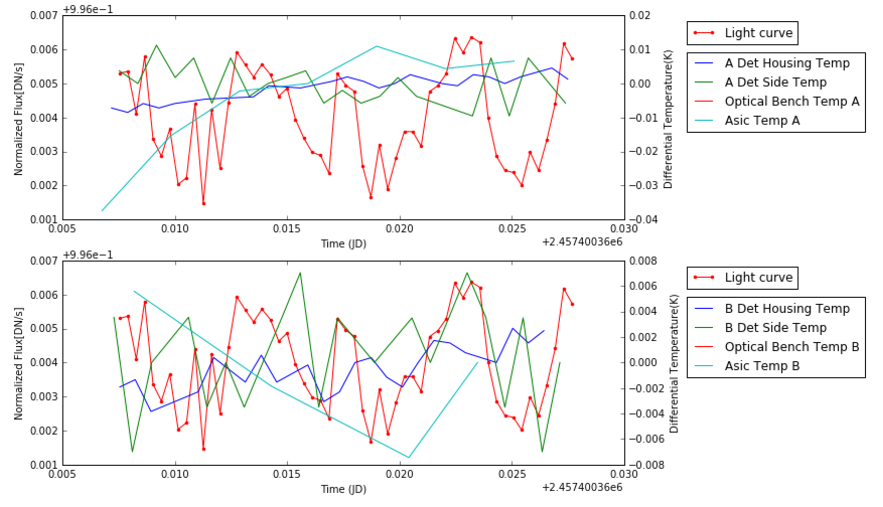
\includegraphics[scale=0.4]{temp_test9}
        \caption{The averaged light curve compared with detector temperatures}
    \end{subfigure}
   
    \begin{subfigure}{3}
        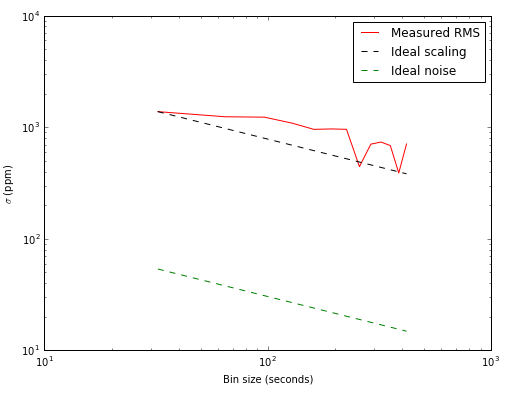
\includegraphics[scale=0.6]{rms_test9}
        \caption{RMS Vs. Bin size}
    \end{subfigure}
    \caption{Analysis of Test 9: FULL6}
\end{figure}


\subsection{Test 10: FULL7} 
\begin{figure}[H]
    \centering
    \begin{subfigure}{1}
        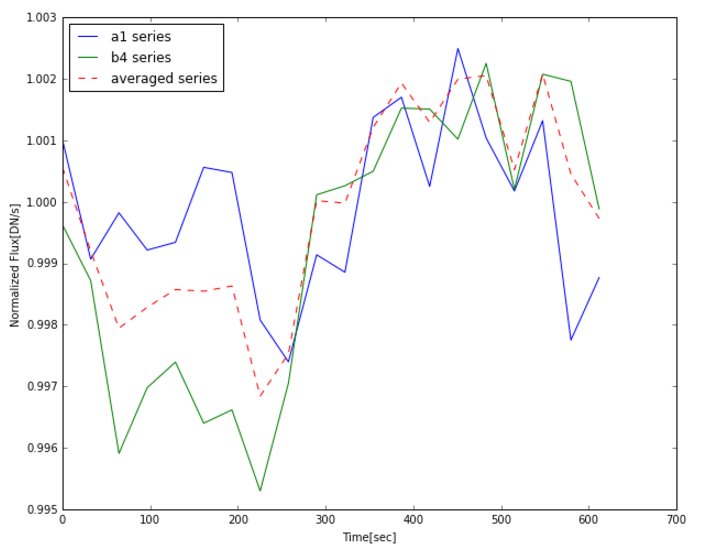
\includegraphics[scale=0.4]{ts_test10}
        \caption{Light curves of a1 series, b4 series and their average}
    \end{subfigure}

    \begin{subfigure}{2}
        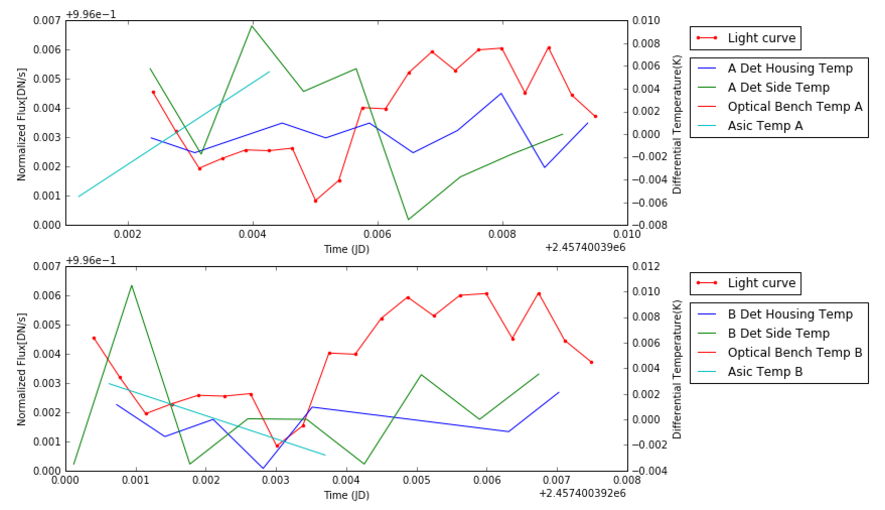
\includegraphics[scale=0.4]{temp_test10}
        \caption{The averaged light curve compared with detector temperatures}
    \end{subfigure}
   
    \begin{subfigure}{3}
        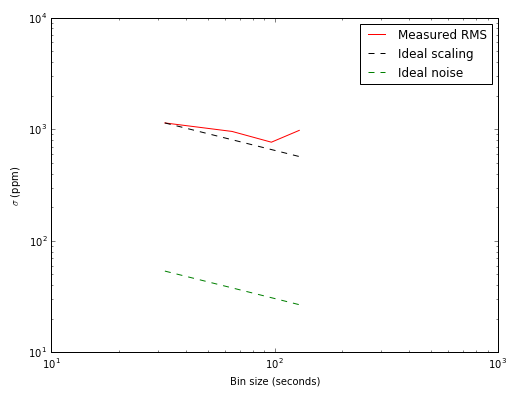
\includegraphics[scale=0.6]{rms_test10}
        \caption{RMS Vs. Bin size}
    \end{subfigure}
    \caption{Analysis of Test 10: FULL7}
\end{figure}


\subsection{Test 11: FULLQ} 
\begin{figure}[H]
    \centering
    \begin{subfigure}{1}
        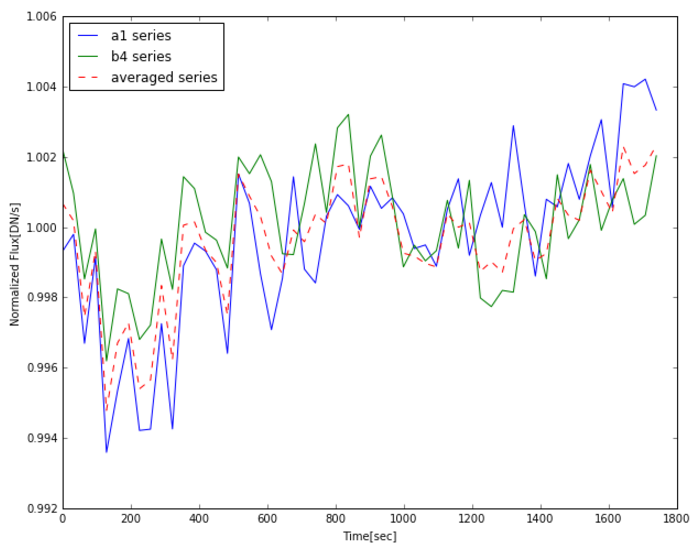
\includegraphics[scale=0.4]{ts_test11}
        \caption{Light curves of a1 series, b4 series and their average}
    \end{subfigure}

    \begin{subfigure}{2}
        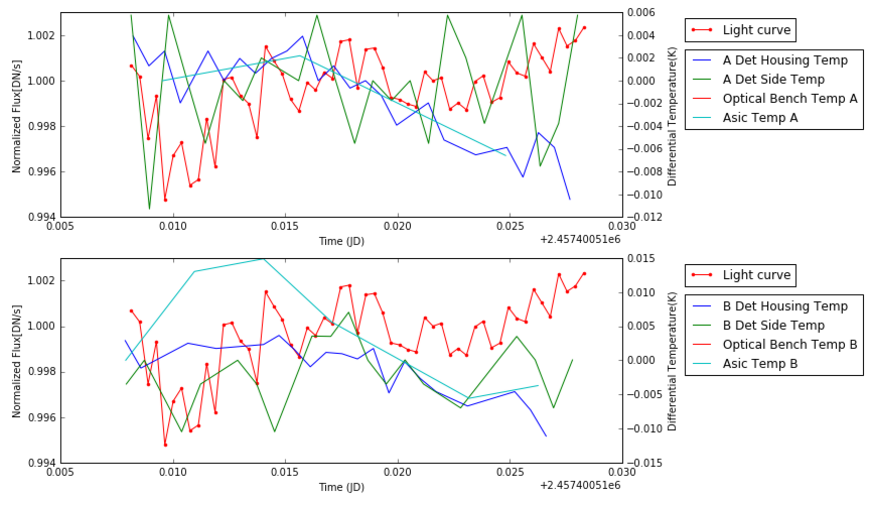
\includegraphics[scale=0.4]{temp_test11}
        \caption{The averaged light curve compared with detector temperatures}
    \end{subfigure}
   
    \begin{subfigure}{3}
        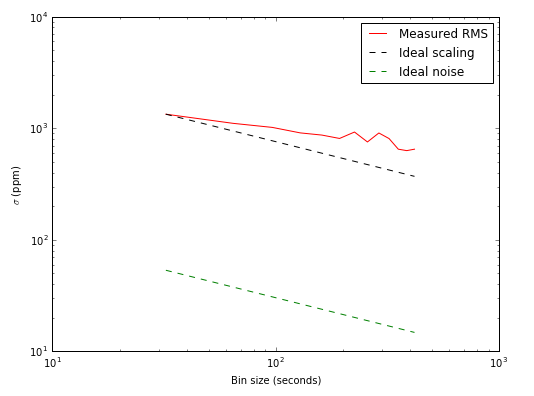
\includegraphics[scale=0.6]{rms_test11}
        \caption{RMS Vs. Bin size}
    \end{subfigure}
    \caption{Analysis of Test 11: FULLQ}
\end{figure}


\subsection{Test 12: FULL9} 
\begin{figure}[H]
    \centering
    \begin{subfigure}{1}
        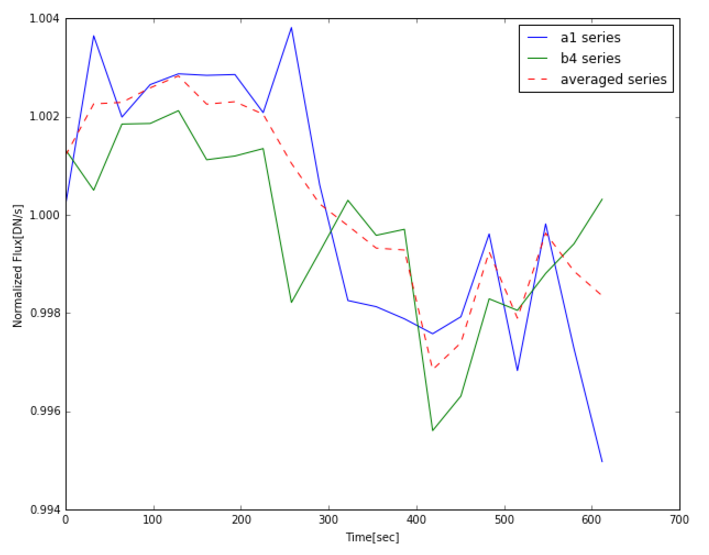
\includegraphics[scale=0.4]{ts_test12}
        \caption{Light curves of a1 series, b4 series and their average}
    \end{subfigure}

    \begin{subfigure}{2}
        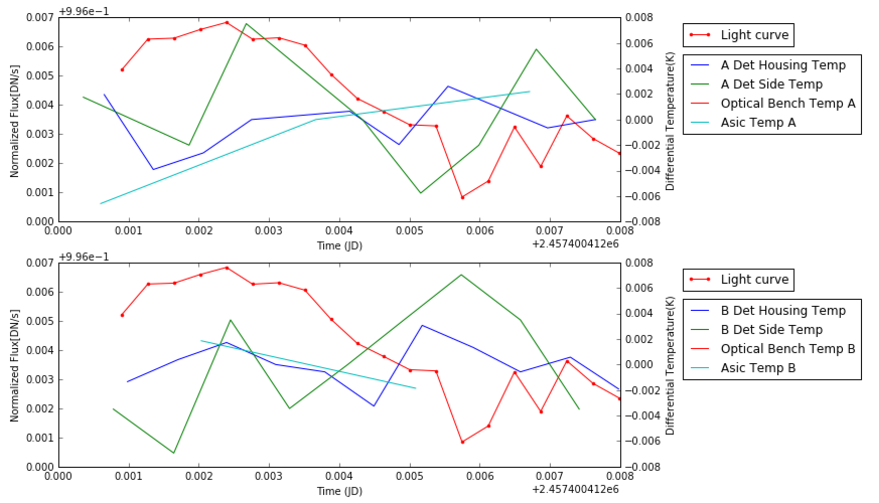
\includegraphics[scale=0.4]{temp_test12}
        \caption{The averaged light curve compared with detector temperatures}
    \end{subfigure}
   
    \begin{subfigure}{3}
        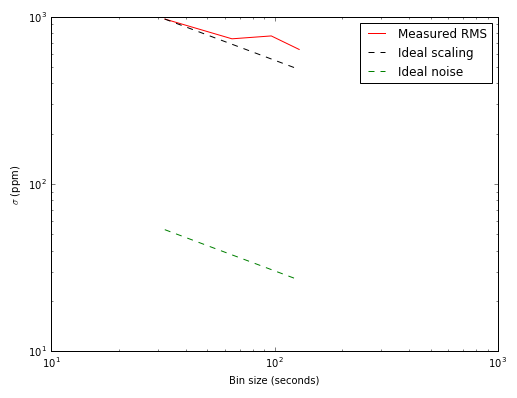
\includegraphics[scale=0.6]{rms_test12}
        \caption{RMS Vs. Bin size}
    \end{subfigure}
    \caption{Analysis of Test 12: FULL9}
\end{figure}


\subsection{Test 13: FULL10} 
\begin{figure}[H]
    \centering
    \begin{subfigure}{1}
        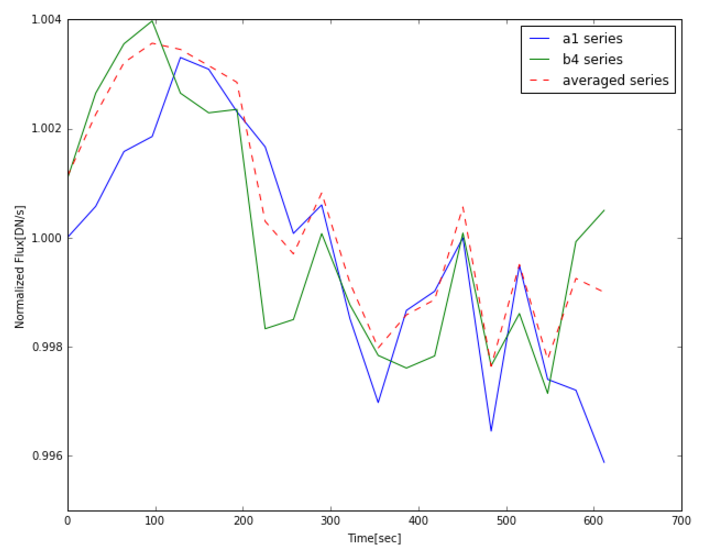
\includegraphics[scale=0.4]{ts_test13}
        \caption{Light curves of a1 series, b4 series and their average}
    \end{subfigure}

    \begin{subfigure}{2}
        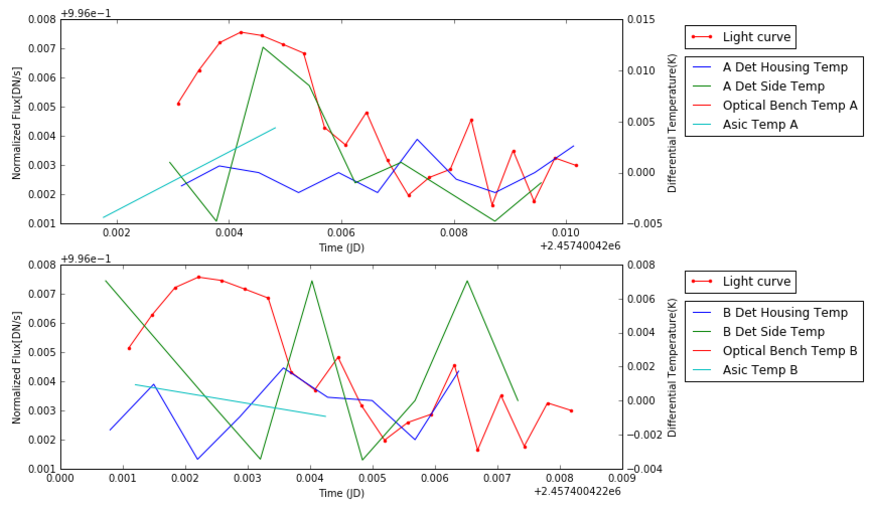
\includegraphics[scale=0.4]{temp_test13}
        \caption{The averaged light curve compared with detector temperatures}
    \end{subfigure}
   
    \begin{subfigure}{3}
        \includegraphics[scale=0.6]{rms_test13}
        \caption{RMS Vs. Bin size}
    \end{subfigure}
    \caption{Analysis of Test 13: FULL10}
\end{figure}


\subsection{Test 14: FULL11} 
\begin{figure}[H]
    \centering
    \begin{subfigure}{1}
        \includegraphics[scale=0.4]{ts_test14}
        \caption{Light curves of a1 series, b4 series and their average}
    \end{subfigure}

    \begin{subfigure}{2}
        \includegraphics[scale=0.4]{temp_test14}
        \caption{The averaged light curve compared with detector temperatures}
    \end{subfigure}
   
    \begin{subfigure}{3}
        \includegraphics[scale=0.6]{rms_test14}
        \caption{RMS Vs. Bin size}
    \end{subfigure}
    \caption{Analysis of Test 14: FULL11}
\end{figure}


\subsection{Test 15: FULL12} 
\begin{figure}[H]
    \centering
    \begin{subfigure}{1}
        \includegraphics[scale=0.4]{ts_test15}
        \caption{Light curves of a1 series, b4 series and their average}
    \end{subfigure}

    \begin{subfigure}{2}
        \includegraphics[scale=0.4]{temp_test15}
        \caption{The averaged light curve compared with detector temperatures}
    \end{subfigure}
   
    \begin{subfigure}{3}
        \includegraphics[scale=0.6]{rms_test15}
        \caption{RMS Vs. Bin size}
    \end{subfigure}
    \caption{Analysis of Test 15: FULL12}
\end{figure}


\subsection{Test 16: FULL13} 
\begin{figure}[H]
    \centering
    \begin{subfigure}{1}
        \includegraphics[scale=0.4]{ts_test16}
        \caption{Light curves of a1 series, b4 series and their average}
    \end{subfigure}

    \begin{subfigure}{2}
        \includegraphics[scale=0.4]{temp_test16}
        \caption{The averaged light curve compared with detector temperatures}
    \end{subfigure}
   
    \begin{subfigure}{3}
        \includegraphics[scale=0.6]{rms_test16}
        \caption{RMS Vs. Bin size}
    \end{subfigure}
    \caption{Analysis of Test 16: FULL13}
\end{figure}


\subsection{Test 17: FULL14} 
\begin{figure}[H]
    \centering
    \begin{subfigure}{1}
        \includegraphics[scale=0.4]{ts_test17}
        \caption{Light curves of a1 series, b4 series and their average}
    \end{subfigure}

    \begin{subfigure}{2}
        \includegraphics[scale=0.4]{temp_test17}
        \caption{The averaged light curve compared with detector temperatures}
    \end{subfigure}
   
    \begin{subfigure}{3}
        \includegraphics[scale=0.6]{rms_test17}
        \caption{RMS Vs. Bin size}
    \end{subfigure}
    \caption{Analysis of Test 17: FULL14}
\end{figure}


\subsection{Test 18: CLRSUB1} 
\begin{figure}[H]
    \centering
    \begin{subfigure}{1}
        \includegraphics[scale=0.4]{ts_test18}
        \caption{Light curves of a1 series, b4 series and their average}
    \end{subfigure}

    \begin{subfigure}{2}
        \includegraphics[scale=0.4]{temp_test18}
        \caption{The averaged light curve compared with detector temperatures}
    \end{subfigure}
   
    \begin{subfigure}{3}
        \includegraphics[scale=0.6]{rms_test18}
        \caption{RMS Vs. Bin size}
    \end{subfigure}
    \caption{Analysis of Test 18: CLRSUB1}
\end{figure}


\subsection{Test 19: CLRSUB2} 
\begin{figure}[H]
    \centering
    \begin{subfigure}{1}
        \includegraphics[scale=0.4]{ts_test19}
        \caption{Light curves of a1 series, b4 series and their average}
    \end{subfigure}

    \begin{subfigure}{2}
        \includegraphics[scale=0.4]{temp_test19}
        \caption{The averaged light curve compared with detector temperatures}
    \end{subfigure}
   
    \begin{subfigure}{3}
        \includegraphics[scale=0.6]{rms_test19}
        \caption{RMS Vs. Bin size}
    \end{subfigure}
    \caption{Analysis of Test 19: CLRSUB2}
\end{figure}


\subsection{Test 20: CLRSUB3} 
\begin{figure}[H]
    \centering
    \begin{subfigure}{1}
        \includegraphics[scale=0.4]{ts_test20}
        \caption{Light curves of a1 series, b4 series and their average}
    \end{subfigure}

    \begin{subfigure}{2}
        \includegraphics[scale=0.4]{temp_test20}
        \caption{The averaged light curve compared with detector temperatures}
    \end{subfigure}
   
    \begin{subfigure}{3}
        \includegraphics[scale=0.6]{rms_test20}
        \caption{RMS Vs. Bin size}
    \end{subfigure}
    \caption{Analysis of Test 20: CLRSUB3}
\end{figure}


\subsection{Test 21: CLRSUB4} 
\begin{figure}[H]
    \centering
    \begin{subfigure}{1}
        \includegraphics[scale=0.4]{ts_test21}
        \caption{Light curves of a1 series, b4 series and their average}
    \end{subfigure}

    \begin{subfigure}{2}
        \includegraphics[scale=0.4]{temp_test21}
        \caption{The averaged light curve compared with detector temperatures}
    \end{subfigure}
   
    \begin{subfigure}{3}
        \includegraphics[scale=0.6]{rms_test21}
        \caption{RMS Vs. Bin size}
    \end{subfigure}
    \caption{Analysis of Test 21: CLRSUB4}
\end{figure}


\subsection{Test 22: CLRSUB5} 
\begin{figure}[H]
    \centering
    \begin{subfigure}{1}
        \includegraphics[scale=0.4]{ts_test22}
        \caption{Light curves of a1 series, b4 series and their average}
    \end{subfigure}

    \begin{subfigure}{2}
        \includegraphics[scale=0.4]{temp_test22}
        \caption{The averaged light curve compared with detector temperatures}
    \end{subfigure}
   
    \begin{subfigure}{3}
        \includegraphics[scale=0.6]{rms_test22}
        \caption{RMS Vs. Bin size}
    \end{subfigure}
    \caption{Analysis of Test 22: CLRSUB5}
\end{figure}


\subsection{Test 23: CLRSUB6} 
\begin{figure}[H]
    \centering
    \begin{subfigure}{1}
        \includegraphics[scale=0.4]{ts_test23}
        \caption{Light curves of a1 series, b4 series and their average}
    \end{subfigure}

    \begin{subfigure}{2}
        \includegraphics[scale=0.4]{temp_test23}
        \caption{The averaged light curve compared with detector temperatures}
    \end{subfigure}
   
    \begin{subfigure}{3}
        \includegraphics[scale=0.6]{rms_test23}
        \caption{RMS Vs. Bin size}
    \end{subfigure}
    \caption{Analysis of Test 23: CLRSUB6}
\end{figure}


\subsection{Test 24: WLP8A1B4} 
\begin{figure}[H]
    \centering
    \begin{subfigure}{1}
        \includegraphics[scale=0.4]{ts_test24}
        \caption{Light curves of a1 series, b4 series and their average}
    \end{subfigure}

    \begin{subfigure}{2}
        \includegraphics[scale=0.4]{temp_test24}
        \caption{The averaged light curve compared with detector temperatures}
    \end{subfigure}
   
    \begin{subfigure}{3}
        \includegraphics[scale=0.6]{rms_test24}
        \caption{RMS Vs. Bin size}
    \end{subfigure}
    \caption{Analysis of Test 24: WLP8A1B4}
\end{figure}


\subsection{Test 25: WLP8A2B3} 
\begin{figure}[H]
    \centering
    \begin{subfigure}{1}
        \includegraphics[scale=0.4]{ts_test25}
        \caption{Light curves of a1 series, b4 series and their average}
    \end{subfigure}

    \begin{subfigure}{2}
        \includegraphics[scale=0.4]{temp_test25}
        \caption{The averaged light curve compared with detector temperatures}
    \end{subfigure}
   
    \begin{subfigure}{3}
        \includegraphics[scale=0.6]{rms_test25}
        \caption{RMS Vs. Bin size}
    \end{subfigure}
    \caption{Analysis of Test 25: WLP8A2B3}
\end{figure}


\subsection{Test 26: WLP8A3B2} 
\begin{figure}[H]
    \centering
    \begin{subfigure}{1}
        \includegraphics[scale=0.4]{ts_test26}
        \caption{Light curves of a1 series, b4 series and their average}
    \end{subfigure}

    \begin{subfigure}{2}
        \includegraphics[scale=0.4]{temp_test26}
        \caption{The averaged light curve compared with detector temperatures}
    \end{subfigure}
   
    \begin{subfigure}{3}
        \includegraphics[scale=0.6]{rms_test26}
        \caption{RMS Vs. Bin size}
    \end{subfigure}
    \caption{Analysis of Test 26: WLP8A3B2}
\end{figure}



\section{Conclusion}
After analyzing the tests, we found that the best way to process the data involves the following methods: 1) Generating separate centers for each image 2) Doing a linear fitting to remove trend 3) Using Slope2 method for files with $NGROUP = 2$ 4) Using annular aperture function rather than median subtraction to subtract background \& 5) Using MMM tests, i.e. apply no correction method  

\end{document}
